%o   Project goal and motivation
%o   Project summary and overview - the "red thread"
%o   Project results (brief summary)
%o   Dissertation Layout
%
%Nytta med projektet, bakomliggande motivering, hypotes kring resultat (Google Glass kommer vara bättre än smartphone eftersom handsfree and stuff), layout av rapporten.
%
%Prata allmänt om vad det finns för problem idag, mer specifikt vad kommer vår applikation att lösa, mixa med frågor som kan besvaras bland slutsatserna
%
%
%

Although assembling components into a fully functional product can be a tedious task, an employee assembling many different products may not be able to learn the process by heart, and will need to rely on instruction manuals.

However, carrying instruction manuals around would mean having to find specific instructions and also, while assembling components, the instructions will have to be placed in the assembler's line of sight. As such, the assembler's focus will have to shift between the components and the instructions, perhaps turn his or her head around, and the assembler may potentially even need to use his or her hands in order to browse the instructions. 

One solution to the problem would be to use a TV or computer screen. For example, instructions could be browsed hands-free using a foot pedal. However, such technology requires the use of both hands and one foot. In other words, it would require some coordination. Although mobile, such technology would also had to be carried around, similar to printed instructions.

Using a smartphone removes the requirement for written instructions on paper and a smartphone is also small enough to be put in a pocket. However, a smartphone still requires touch operations and as such will occupy at least one of the assembler's hands at some point. A smartphone, similar to ring binders, will also have to be placed in the assembler's line of sight.

New technology may offer a better solution. Google Glass is a computational device, which looks like, and is worn as, regular glass frames~\cite{glassStart}. Google Glass also has a display positioned slightly above the user's line of sight, meaning that the Google Glass display is always in the assembler's line of sight. Google Glass can also be entirely controlled via voice commands, meaning that the user may operate Google Glass completely hands-free.

This dissertation describes the design, implementation and evaluation of an application for Google Glass. In this project, the application will enable users to scan a quick response (QR) code related to a specific product and get information on which components are needed to assemble the specific product, as well as instructions on how to assemble the components.

The application will also be built for smartphones, giving a reference point for the evaluation as well as a method of comparison with the Google Glass application. The reason for comparing the Google Glass application with a smartphone application is because smartphone are small and mobile, similar to Google Glass. Using the Google Glass application, users will be able to assemble products by following instructions, without having to shift their focus from what they are doing, and neither will the users have to use their hands in order to control the application.

The application, described in Figure~\ref{projectmapLightVersion}, will scan a QR code, download information from a database based on the information received from the QR code, and then display the downloaded information in the form of a slide view. The application will exist in two versions, one for Google Glass and another for smartphones. However, they will both function in the same way and as such the device in Figure~\ref{projectmapLightVersion} could be either Google Glass or a smartphone.

	\begin{figure}[ht!]
		\centering
		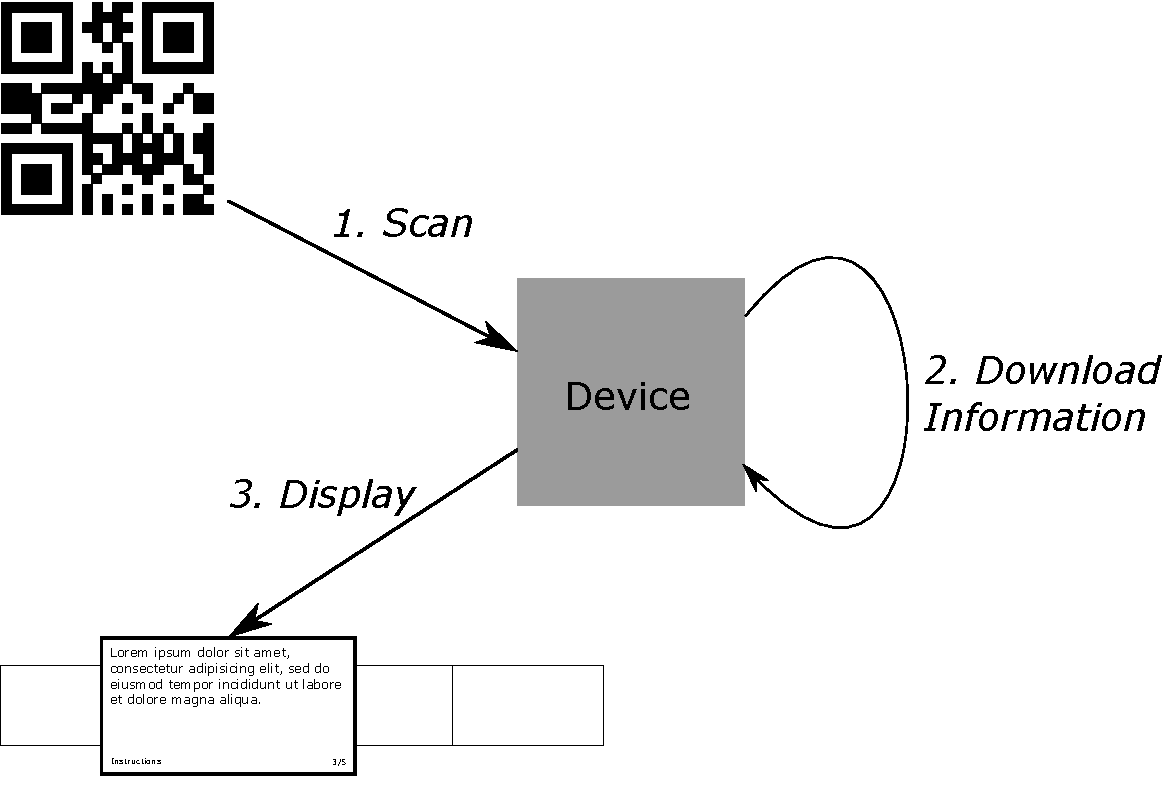
\includegraphics[width=110mm]{images/projectmapLightVersion}
		\caption{Application functionality.}
		\label{projectmapLightVersion}
	\end{figure}
	
The project was specified by, and implemented at, Sogeti Karlstad. Sogeti is an IT consulting company with focus on competence and modern technology. Since Sogeti works with applications for mobile plattforms, and one of the latest mobile technologies are Google Glass, evaluating the new technology and the potential customer use is of interest to Sogeti. The full project specification, although written in Swedish, can be found in Appendix~\ref{app:projectspec}.

\subsection{Discontinuance of the Explorer Program}
It should be noted that, since this dissertation began, Google has chosen to cancel the so called ``explorer program'' for Google Glass~\cite{glassDiscontinued}. The explorer program was the ``open beta phase'' of Google Glass where Google, although Google Glass was sold as a consumer product, was still developing Google Glass at Google's research center, called Google X. Google used users' input and feedback to improve on Google Glass as a product, both in terms of hardware and software.

Now, at the end of the open beta phase, Google has chosen to keep developing Google Glass, but without the help of consumers, meaning that any further updates, both in terms of hardware as well as software, will (as of now) not be publicly available. When discussing the future of Google Glass, Google stated that the company is ``thrilled to be moving even more from concept to reality''. As of January 20th, 2015, the Google Glass Explorer Edition was no longer available for sale. However, Google ensures that Google Glass will return ``when they're ready'', but does not go in to further details on when Google Glass will be available for sale again or what the new version will entail. 

\subsection{Back-End}
The original project, of which this dissertation is a part, was divided in to two different parts. This dissertation will cover the front-end part of the project, which includes building the application, both the Google Glass version and the smartphone version. This dissertation will also discuss the different ways of presenting information and how information is presented in the application.

However, the second part of the project is the back-end part. The back-end part has been summed up in Figure~\ref{projectmapLightVersion} as ``Download Information''. The back-end part was implemented by Richard Hoorn and consists of a web application programming interface (API), connected to a database in which all product information is stored~\cite{hoorn}. 

\subsection{Expected Results}
The expected result is that the Google Glass application will prove useful and valuable, more so than the smartphone application. In terms of test results, Google Glass is expected to be on par with the smartphone equivalents. Since the features of Google Glass are their selling points, performing better than, or equal to, smartphones would give a strong argument why Google Glass would be better than smartphones for assembly instructions.

However, should Google Glass perform worse than smartphones in some or all of the tests, Google Glass could still be deemed the better option due to its features. The hands-free aspect of Google Glass is a strong enough argument in itself why Google Glass should be preferred over smartphones. 

%As such Google Glass could be deemed the better option over smartphones despite potentially worse results in comparison to smartphones. Google Glass is not expected to perform better than smartphones, but only to be reasonably behind smartphones, giving weight to the argument that Google Glass should be used in order to make the assembling of components an easier task. The difference in time should be such that the task to be performed does not take significantly longer to perform when using Google Glass in comparison to using a smartphone, taking in to account the hands-free aspect of Google Glass.

In terms of the text length Google Glass may fit on screen Google Glass can not be expected to fit the same amount of information on screen as smartphones. The Google Glass screen is smaller than the screen on smartphones available on the market around the time that Google Glas was released (2013). For Google Glass to be considered the better option in terms of the amount of information that may fit on screen, the difference in the amount of information Google Glass is able to display, in comparison to smartphones, should be such that it would still be possible to deliver the necessary information to the user.

\subsection{Project Results}
The results show that Google Glass is almost always slower, both in terms of decoding the QR code and presenting the information to the user. On average Google Glass is about half a second slower than smartphone equivalents. In terms of the amount of information that may be displayed on the Google Glass display compared to the display on smartphones it was shown that the same amount of text that filled the screen on a smartphone needed three to four separate screens on Google Glass.

\subsection{Dissertation Layout}
Chapter~\ref{sec:background} discusses the relevant background information regarding Google Glass. The chapter will include an introduction to what Google Glass is, how the device came about and what features it has. The background chapter will also discuss similar products to Google Glass, as well as compare Google Glass to smartphones. Finally, chapter~\ref{sec:background} will include some discussion on topics relevant to the project, including QR code and ways of presenting information.

Chapter~\ref{sec:design} is about the design of the project. The discussion revolves around how the application is intended to work, and what limitations may apply to the implementation of the application, both on Google Glass and smartphone. Chapter~\ref{sec:design} also discusses the design of the tests carried out on the application.

Chapter~\ref{sec:implementation} describes the implementation part of the project. The flow of the application is described in detail. Specific aspects of the application are also described in more detail, such as the layout of the slides as well as the voice commands. The experimental setup and how the tests were performed is also described here.

In chapter~\ref{sec:resultevaluation} the results of the tests are presented. The results are presented along with comments regarding their interpretation as well as comments on any potential error factors during testing.

The final chapter, chapter~\ref{sec:conclusion}, contains conclusions on the project, including conclusions with regard to the test results, as well as conclusions on the project as a whole. Chapter six also includes comments based on personal user experience from using Google Glass for about three months. Finally future work is discussed and the dissertation is concluded with some concluding remarks.

Attached to the dissertation, after the reference list, are appendices. In appendix~\ref{sec:abbreviations} abbreviations used throughout the dissertation are listed. Appendix~\ref{app:results} shows all the individual test results. Appendix~\ref{app:code}, although namned Code, does not contain the project code, but rather a reference to a separate file containing the code, as there is simply too much code to fit in the dissertation. Appendix~\ref{app:projectspec} is the last appendix and contains the original project specification, written in Swedish.